\section{Implications for Higgs and weak boson production}
\label{sec:pheno}

The reduction of PDF uncertainties made possible by neutrino DIS measurements
at the FPF, discussed in Sect.~\ref{sec:protonPDFs},
enables more precise theoretical predictions for core processes at the
HL-LHC.
%
Here we present an initial study of the phenomenological implications
of the PDFs enhanced with LHC neutrino data
for hard-scattering processes at proton colliders.
%
Specifically, we present results for 
single and double gauge boson production,  Higgs production in
vector-boson fusion, and Higgs production and in association with a vector boson.
%
We focus on processes sensitive to the quark-quark and quark-antiquark initial
states, given that LHC neutrinos do not provide information on the gluon
PDF and hence they cannot inform  gluon-initiated
processes, such as top quark pair production or Higgs production in gluon fusion.

We adopt the same calculational settings as in the LHC phenomenology analysis considered
in the PDF4LHC21 combination study~\cite{PDF4LHCWorkingGroup:2022cjn} and provide predictions
both for inclusive cross-sections, integrated in the fiducial
region, and for differential distributions.
%
We evaluate these cross-sections using matrix elements
which include NLO corrections both in the
QCD and electroweak coupling using
{\sc\small mg5\_amc@nlo}~\cite{Frederix:2018nkq}
interfaced to {\sc\small PineAPPL}~\cite{Carrazza:2020gss}.
%
For all processes, realistic selection and acceptance cuts on the final state particles
have been applied.
%
No further theory uncertainties are considered in this
analysis, given that we don't aim to compare with experimental data.

%%%%%%%%%%%%%%%%%%%%%%%%%%%%%%%%%%%%%%%%%%%%%%%%%%%%%%%%%%%%%%%%%%%%%%%%
\begin{figure}[htbp]
\centering
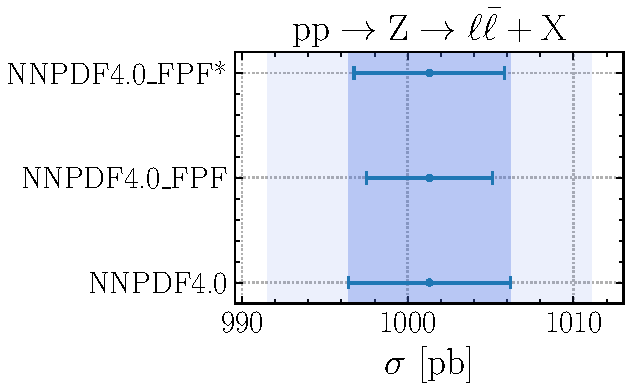
\includegraphics[width=0.32\textwidth]{plots/LHCpheno/NNPDF_DY_14TEV_40_PHENO-integrated.pdf}
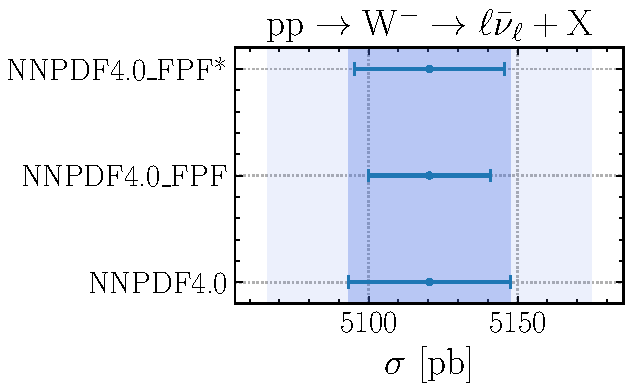
\includegraphics[width=0.32\textwidth]{plots/LHCpheno/NNPDF_WM_14TEV_40_PHENO-integrated.pdf}
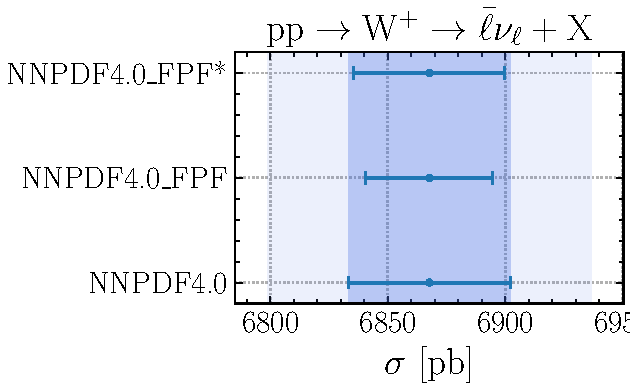
\includegraphics[width=0.32\textwidth]{plots/LHCpheno/NNPDF_WP_14TEV_40_PHENO-integrated.pdf}
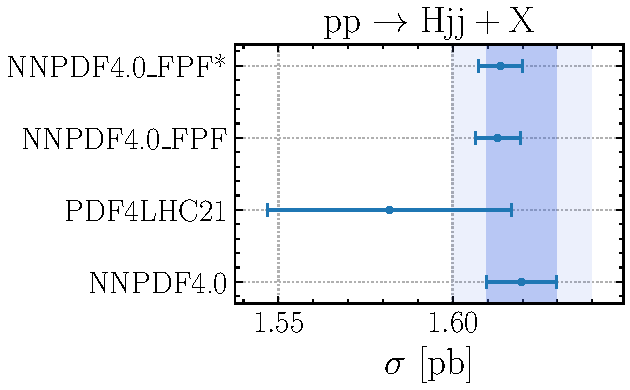
\includegraphics[width=0.32\textwidth]{plots/LHCpheno/NNPDF_HVBF_14TEV_40_PHENO-integrated.pdf}
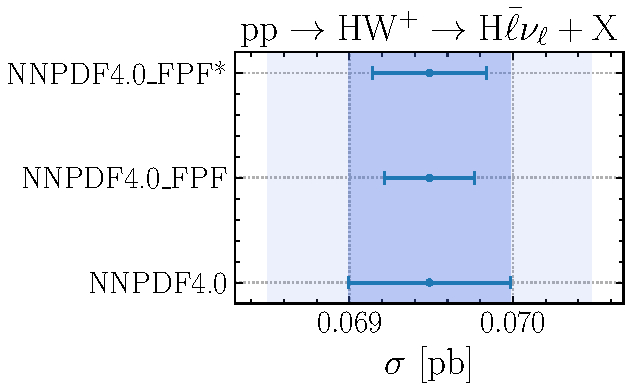
\includegraphics[width=0.32\textwidth]{plots/LHCpheno/NNPDF_HWP_14TEV_40_PHENO-integrated.pdf}
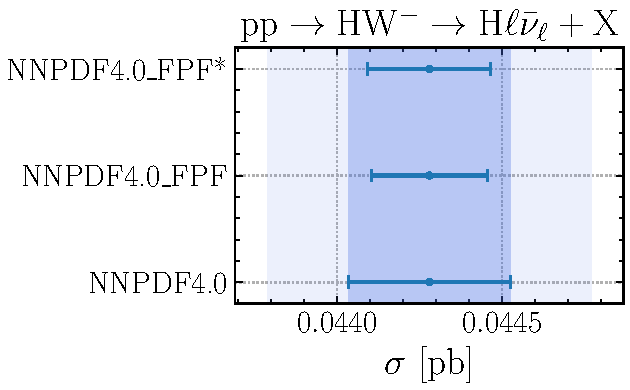
\includegraphics[width=0.32\textwidth]{plots/LHCpheno/NNPDF_HWM_14TEV_40_PHENO-integrated.pdf}
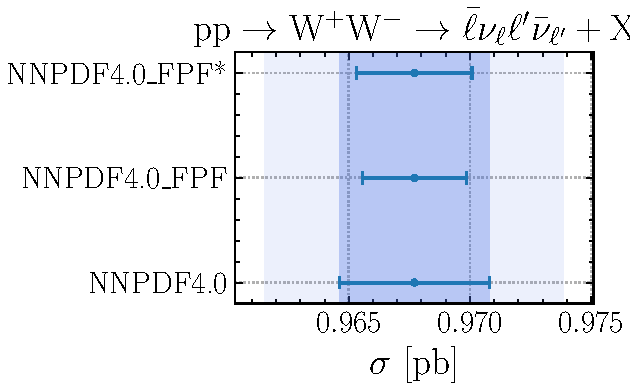
\includegraphics[width=0.32\textwidth]{plots/LHCpheno/NNPDF_WPWM_14TEV_40_PHENO-integrated.pdf}
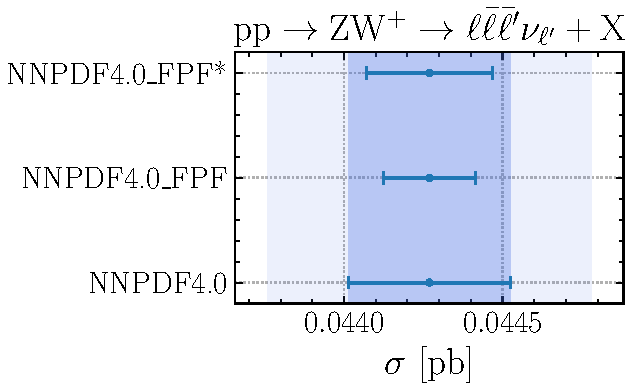
\includegraphics[width=0.32\textwidth]{plots/LHCpheno/NNPDF_WPZ_14TEV_40_PHENO-integrated.pdf}
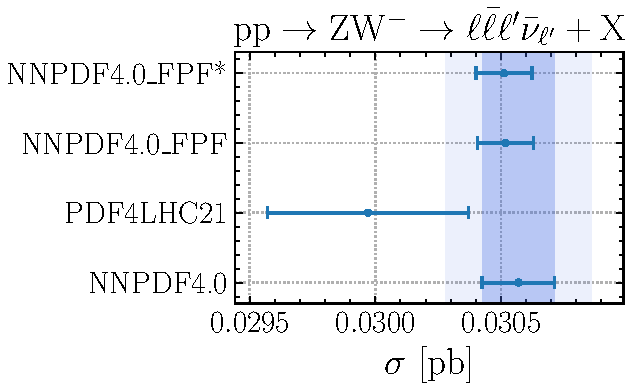
\includegraphics[width=0.32\textwidth]{plots/LHCpheno/NNPDF_WMZ_14TEV_40_PHENO-integrated.pdf}
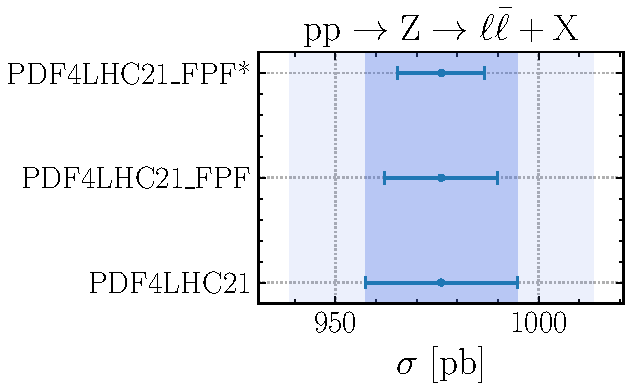
\includegraphics[width=0.32\textwidth]{plots/LHCpheno/NNPDF_DY_14TEV_40_PHENO-integrated-pdf4lhc21.pdf}
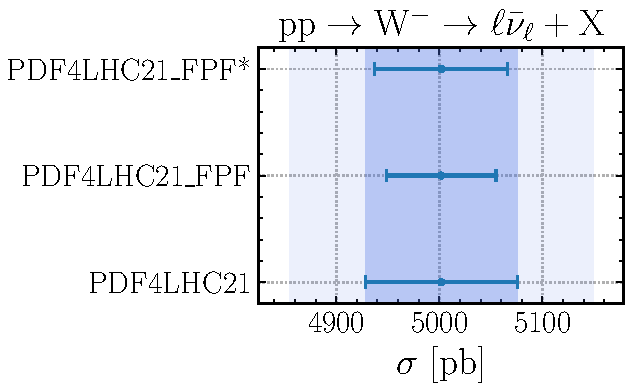
\includegraphics[width=0.32\textwidth]{plots/LHCpheno/NNPDF_WM_14TEV_40_PHENO-integrated-pdf4lhc21.pdf}
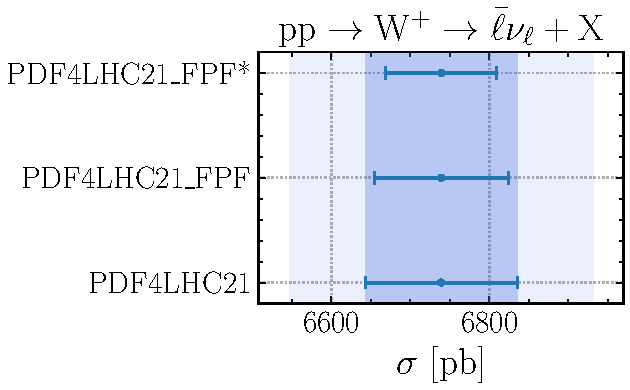
\includegraphics[width=0.32\textwidth]{plots/LHCpheno/NNPDF_WP_14TEV_40_PHENO-integrated-pdf4lhc21.pdf}
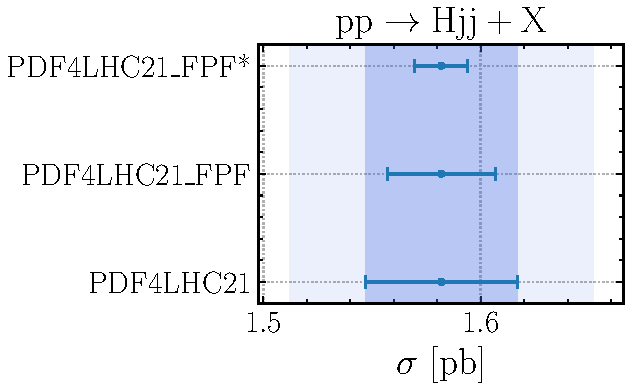
\includegraphics[width=0.32\textwidth]{plots/LHCpheno/NNPDF_HVBF_14TEV_40_PHENO-integrated-pdf4lhc21.pdf}
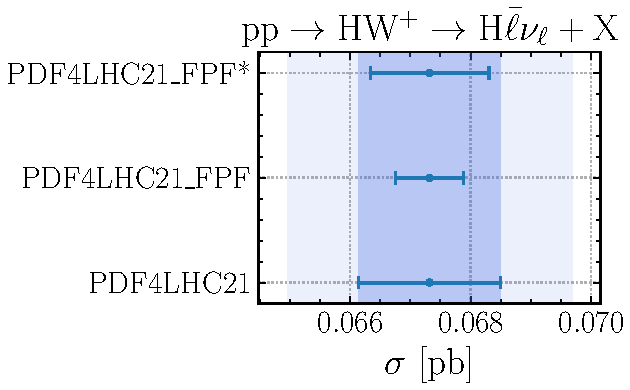
\includegraphics[width=0.32\textwidth]{plots/LHCpheno/NNPDF_HWP_14TEV_40_PHENO-integrated-pdf4lhc21.pdf}
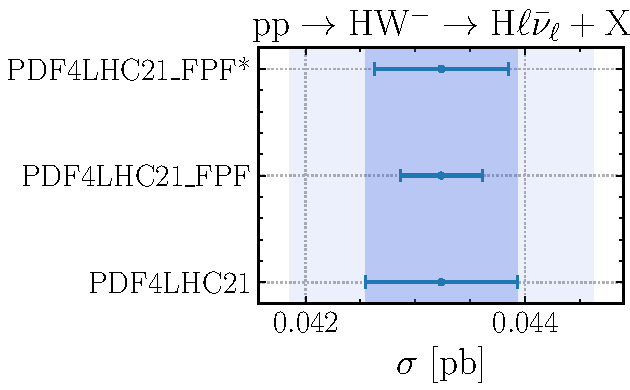
\includegraphics[width=0.32\textwidth]{plots/LHCpheno/NNPDF_HWM_14TEV_40_PHENO-integrated-pdf4lhc21.pdf}
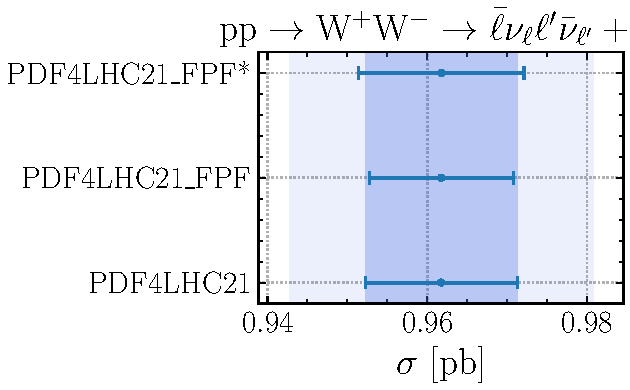
\includegraphics[width=0.32\textwidth]{plots/LHCpheno/NNPDF_WPWM_14TEV_40_PHENO-integrated-pdf4lhc21.pdf}
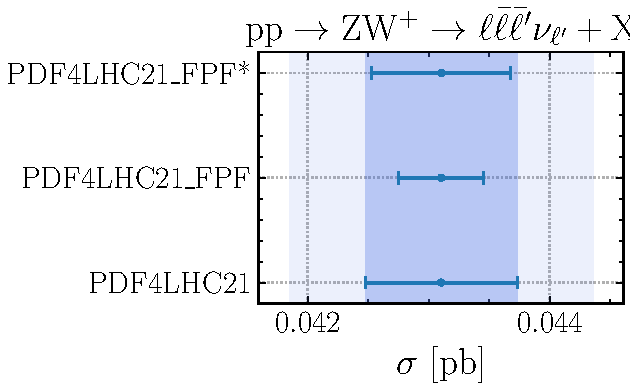
\includegraphics[width=0.32\textwidth]{plots/LHCpheno/NNPDF_WPZ_14TEV_40_PHENO-integrated-pdf4lhc21.pdf}
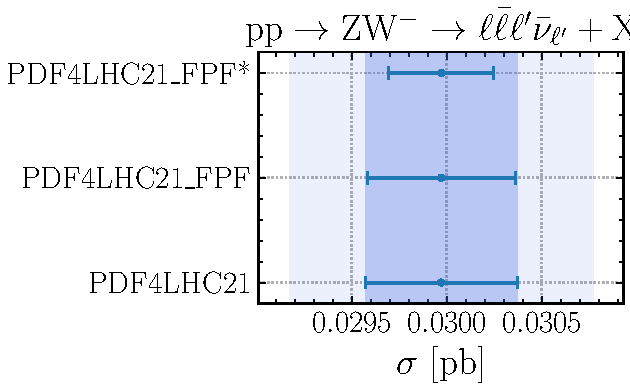
\includegraphics[width=0.32\textwidth]{plots/LHCpheno/NNPDF_WMZ_14TEV_40_PHENO-integrated-pdf4lhc21.pdf}
\caption{Fiducial cross-sections for representative LHC processes at $\sqrt{s}=14$ TeV
  evaluated with NNPDF4.0 (upper panels) and PDF4LHC21 (bottom panels),
  compared with the fits including the FPF structure function projections.
  %
  See~\cite{NNPDF:2021njg,PDF4LHCWorkingGroup:2022cjn} for the calculational settings
  used to evaluate these cross-sections.
%
For the baseline
predictions, the dark (light) bands indicate the 68\% (95\%) CL uncertainties.
%
The fits labelled as ``\_FPF'' are the ones considering statistical uncertainties,
while those labelled as ``\_FPF$^*$'' also include systematic errors.
%
In the fits with FPF data, the central values are set to be the same as
in the corresponding baseline.
%
We provide predictions for inclusive Drell-Yan production ($Z, W^+, W^-$), Higgs production
in vector-boson fusion, Higgs associated
production, and diboson production ($W^+W^-$, $W^+Z$, $W^-Z$).
%
}
\label{fig:NNPDF40_pheno_integrated}
\end{figure}
%%%%%%%%%%%%%%%%%%%%%%%%%%%%%%%%%%%%%%%%%%%%%%%%%%%%%%%%%%%%%%%%%%%%%%%%

Fig.~\ref{fig:NNPDF40_pheno_integrated} displays
fiducial cross-section for representative LHC processes at $\sqrt{s}=14$ TeV
evaluated with NNPDF4.0 (top panels)
and with PDF4LHC21 (bottom panels),
compared with the results obtained from
the corresponding fits including the FPF structure function projections.
%
For the fits with FPF data we display the variants where the covariance matrix
consists only of statistical errors (``\_FPF'') and where also
systematic errors are accounted for (``\_FPF$^*$'').
%
For the baseline
predictions, the dark (light) bands indicate the 68\% (95\%) CL uncertainties.
%
The central values are set to be the same as in the baseline calculation in all cases.
%
From top to bottom, we show inclusive Drell-Yan production in the $Z$, $W^+$, and $W^-$
channels, Higgs production
in vector-boson fusion, Higgs associated
production, and diboson production in the $W^+W^-$, $W^+Z$, and $W^-Z$ final-states.
%
The corresponding comparisons at the level of differential distributions
are shown in Figs.~\ref{fig:NNPDF40_pheno_differential} and~\ref{fig:PDF4LHC21_pheno_differential}
for NNPDF4.0 and PDF4LHC21 respectively.
%
As done for the fiducial cross-sections of Fig.~\ref{fig:NNPDF40_pheno_integrated},
we only indicate the relative PDF uncertainty in each fit.

%%%%%%%%%%%%%%%%%%%%%%%%%%%%%%%%%%%%%%%%%%%%%%%%%%%%%%%%%%%%%%%%%%%%%%%%
\begin{figure}[htbp]
\centering
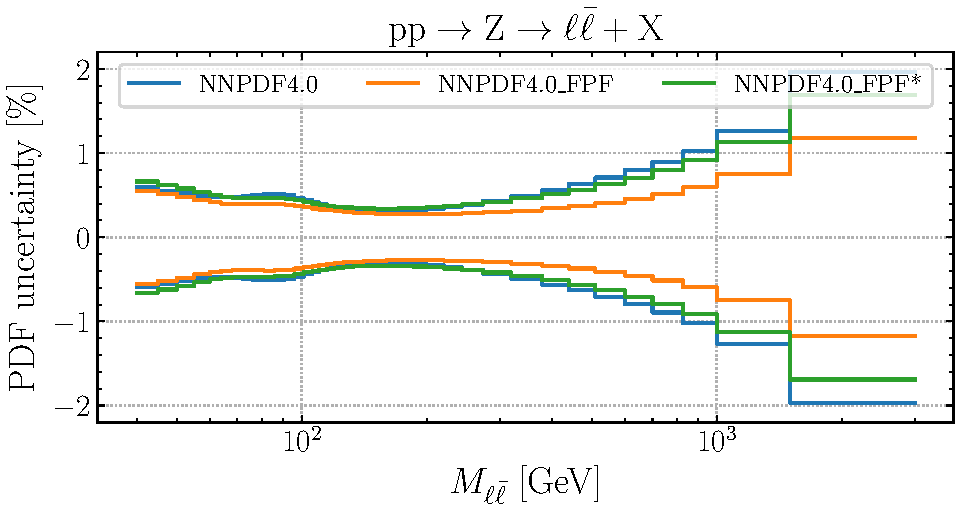
\includegraphics[width=0.49\textwidth]{plots/LHCpheno/NNPDF_DY_14TEV_40_PHENO-global.pdf}
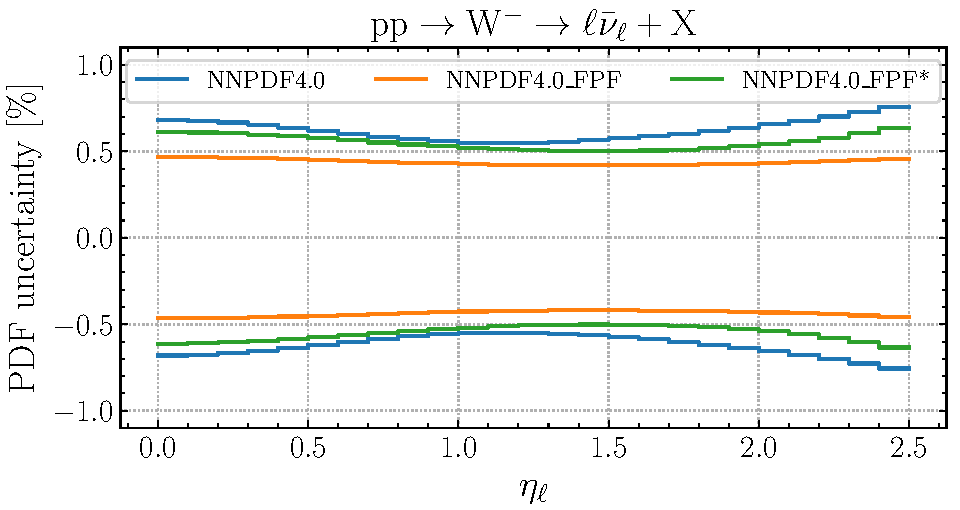
\includegraphics[width=0.49\textwidth]{plots/LHCpheno/NNPDF_WM_14TEV_40_PHENO-global.pdf}
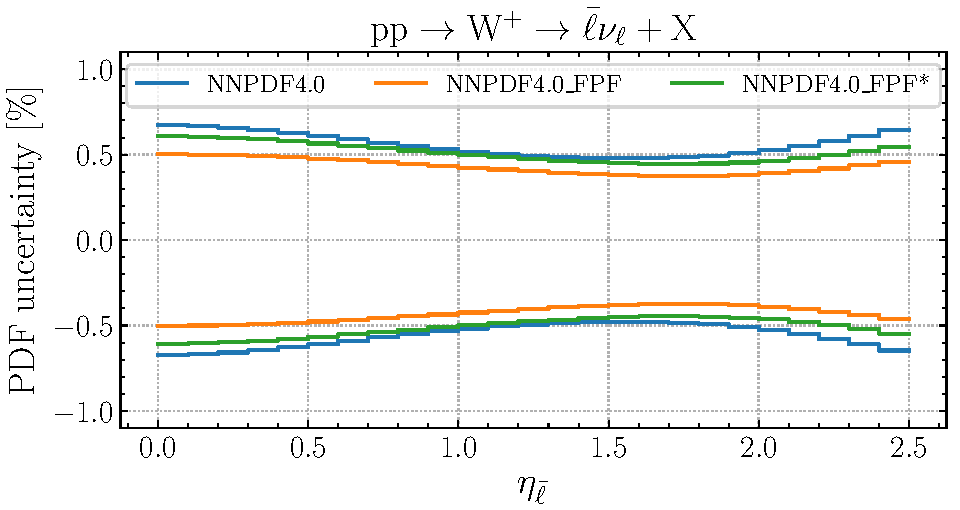
\includegraphics[width=0.49\textwidth]{plots/LHCpheno/NNPDF_WP_14TEV_40_PHENO-global.pdf}
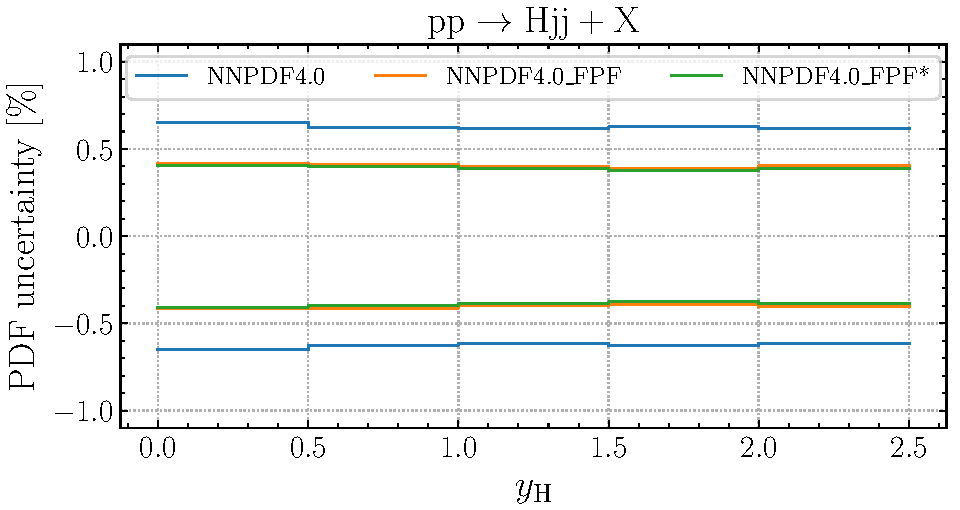
\includegraphics[width=0.49\textwidth]{plots/LHCpheno/NNPDF_HVBF_14TEV_40_PHENO-global.pdf}
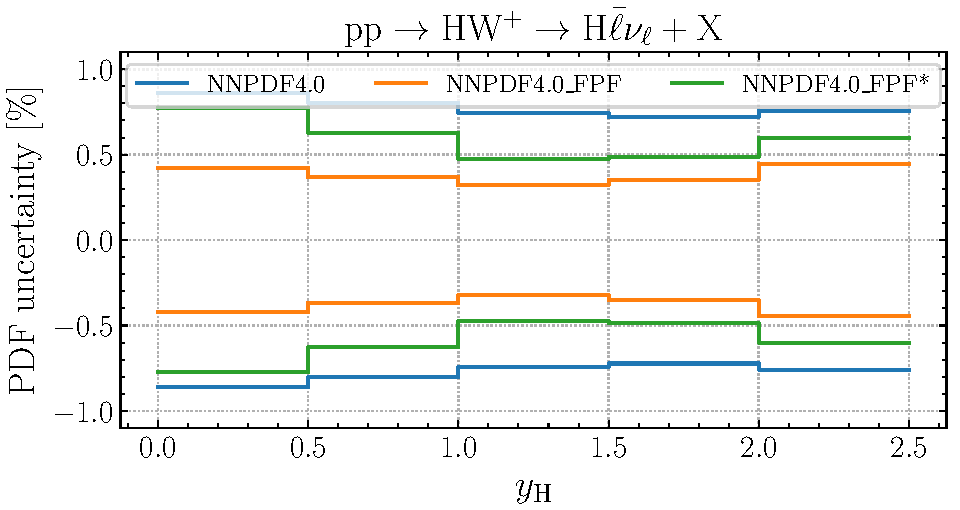
\includegraphics[width=0.49\textwidth]{plots/LHCpheno/NNPDF_HWP_14TEV_40_PHENO-global.pdf}
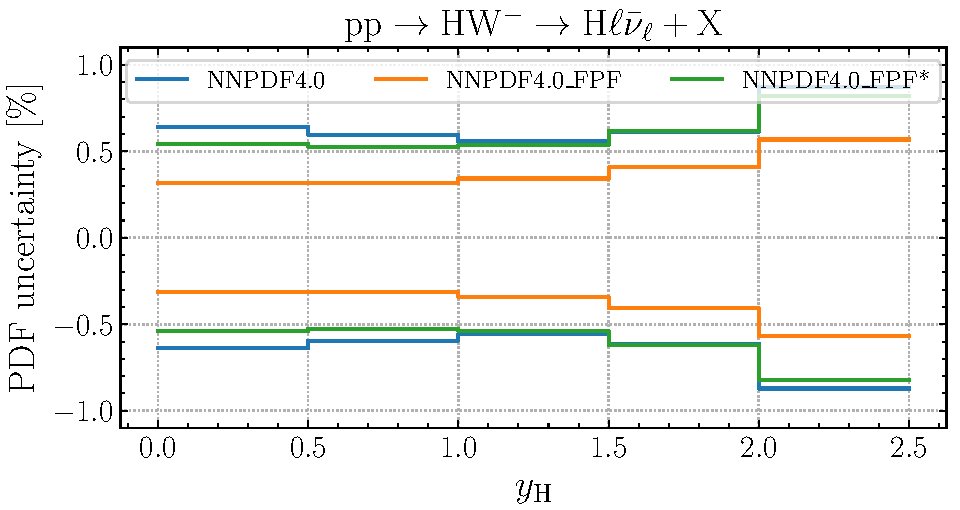
\includegraphics[width=0.49\textwidth]{plots/LHCpheno/NNPDF_HWM_14TEV_40_PHENO-global.pdf}
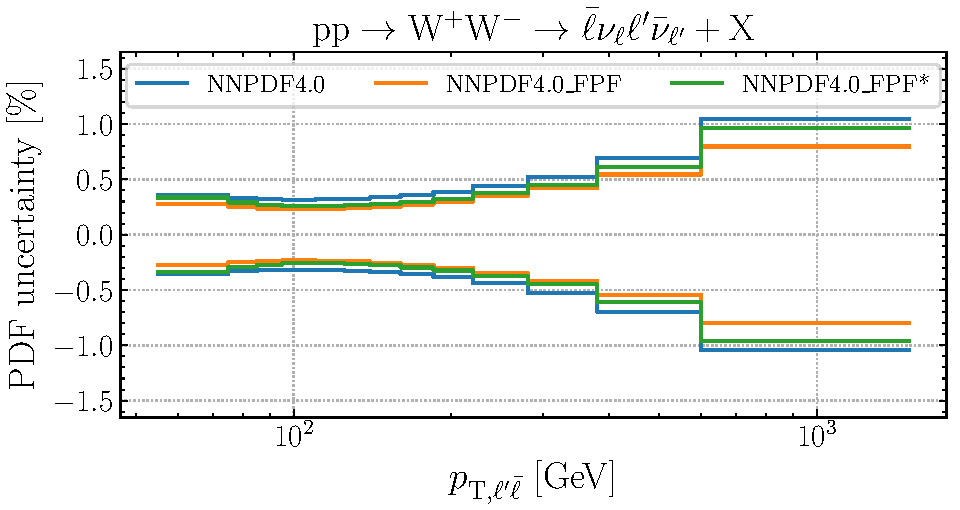
\includegraphics[width=0.49\textwidth]{plots/LHCpheno/NNPDF_WPWM_14TEV_40_PHENO-global.pdf}
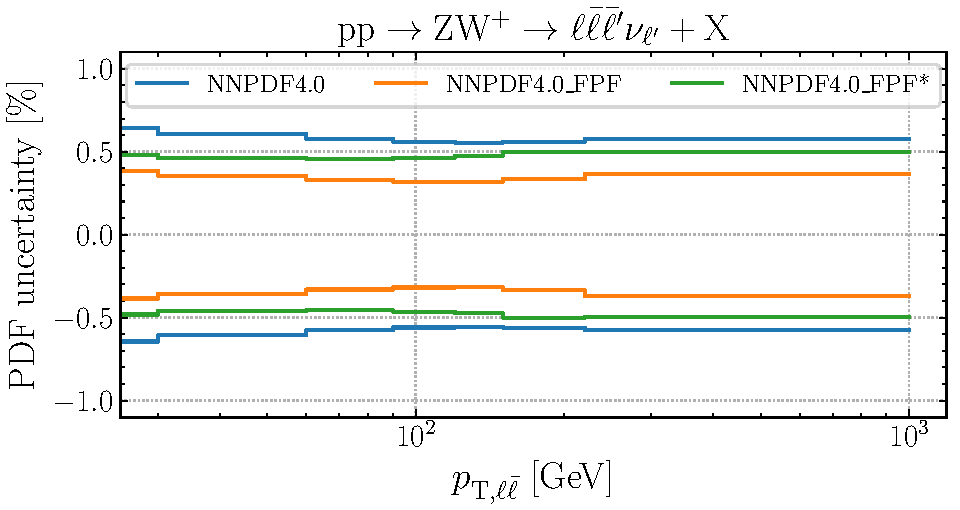
\includegraphics[width=0.49\textwidth]{plots/LHCpheno/NNPDF_WPZ_14TEV_40_PHENO-global.pdf}
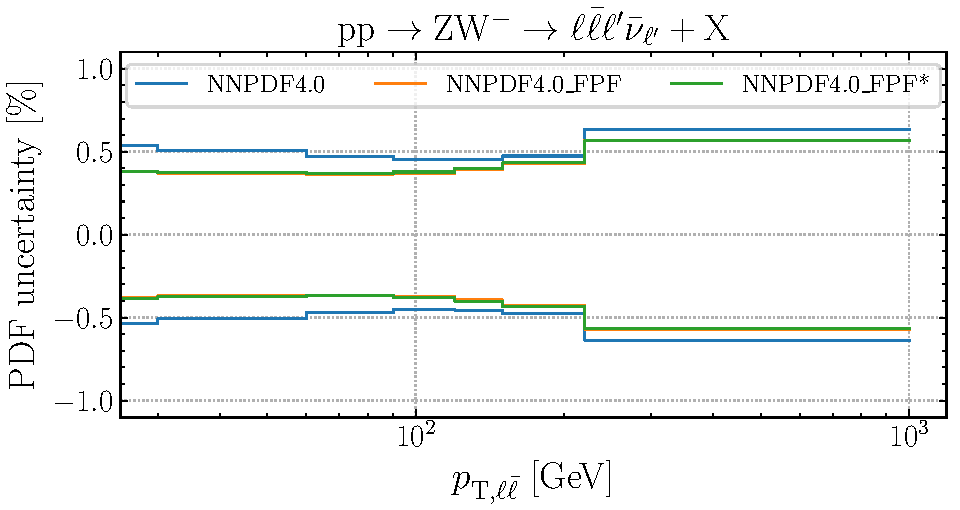
\includegraphics[width=0.49\textwidth]{plots/LHCpheno/NNPDF_WMZ_14TEV_40_PHENO-global.pdf}
\caption{Same as Fig.~\ref{fig:NNPDF40_pheno_integrated}
for the corresponding differential distributions in the case of NNPDF4.0
%
}
\label{fig:NNPDF40_pheno_differential}
\end{figure}
%%%%%%%%%%%%%%%%%%%%%%%%%%%%%%%%%%%%%%%%%%%%%%%%%%%%%%%%%%%%%%%%%%%%%%%%

%%%%%%%%%%%%%%%%%%%%%%%%%%%%%%%%%%%%%%%%%%%%%%%%%%%%%%%%%%%%%%%%%%%%%%%%
\begin{figure}[htbp]
	\centering
	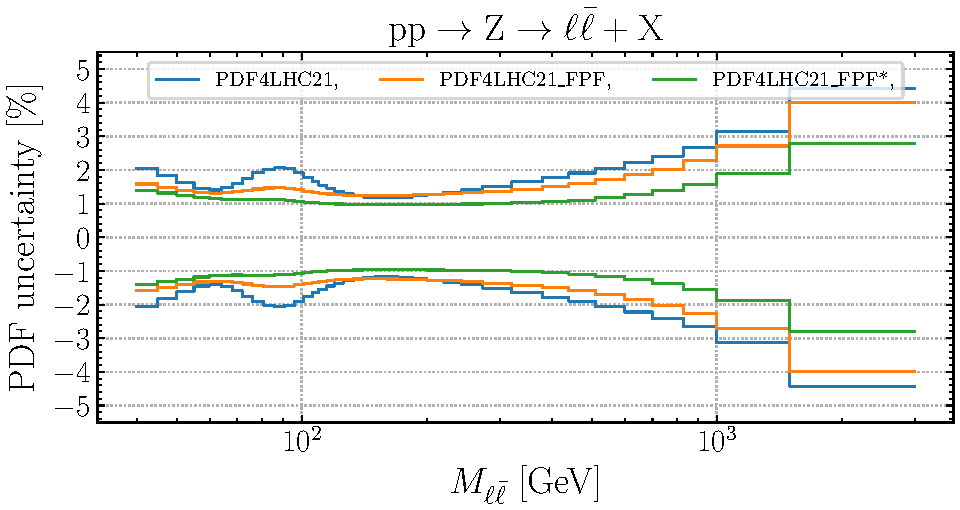
\includegraphics[width=0.49\textwidth]{plots/LHCpheno/NNPDF_DY_14TEV_40_PHENO-global-pdf4lhc21.pdf}
	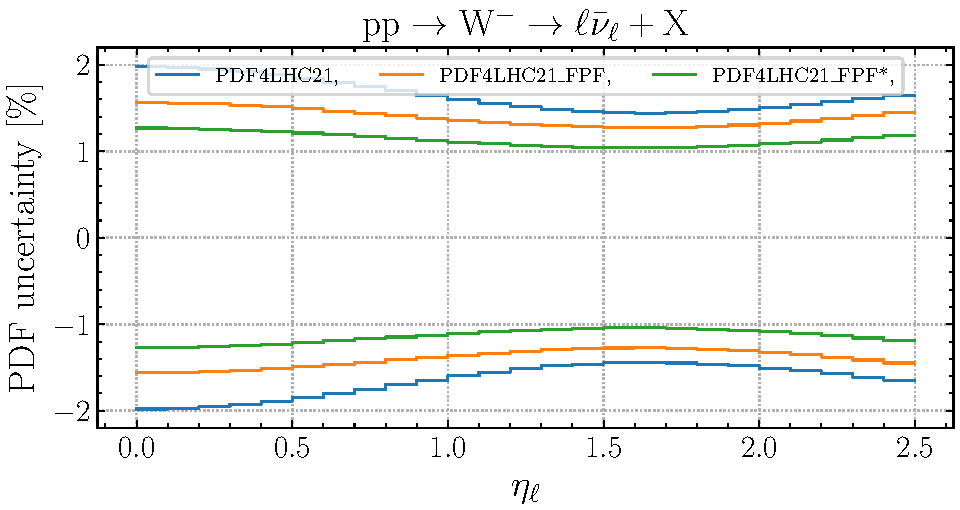
\includegraphics[width=0.49\textwidth]{plots/LHCpheno/NNPDF_WM_14TEV_40_PHENO-global-pdf4lhc21.pdf}
	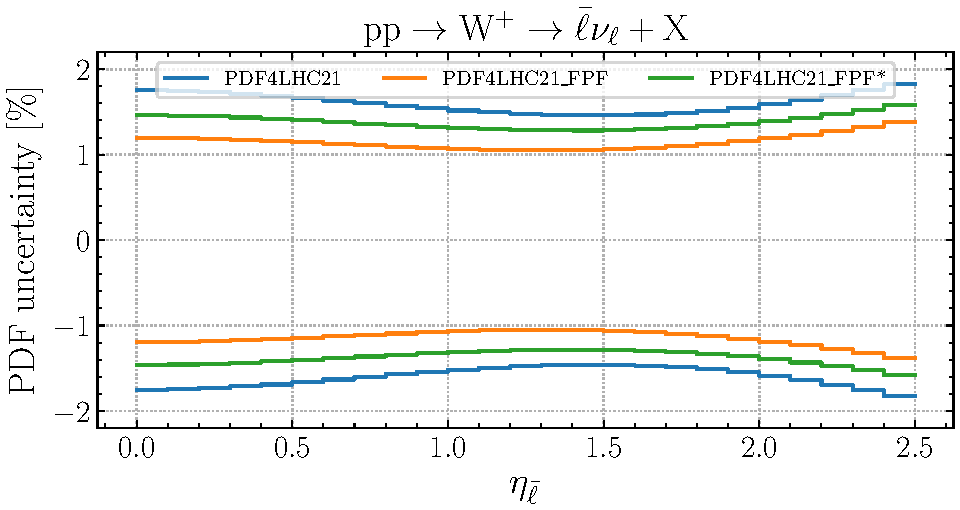
\includegraphics[width=0.49\textwidth]{plots/LHCpheno/NNPDF_WP_14TEV_40_PHENO-global-pdf4lhc21.pdf}
	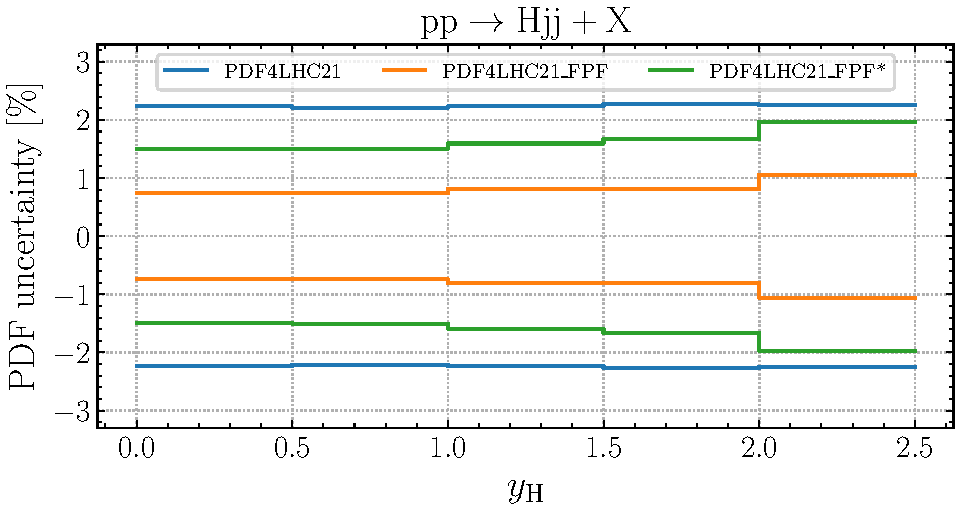
\includegraphics[width=0.49\textwidth]{plots/LHCpheno/NNPDF_HVBF_14TEV_40_PHENO-global-pdf4lhc21.pdf}
	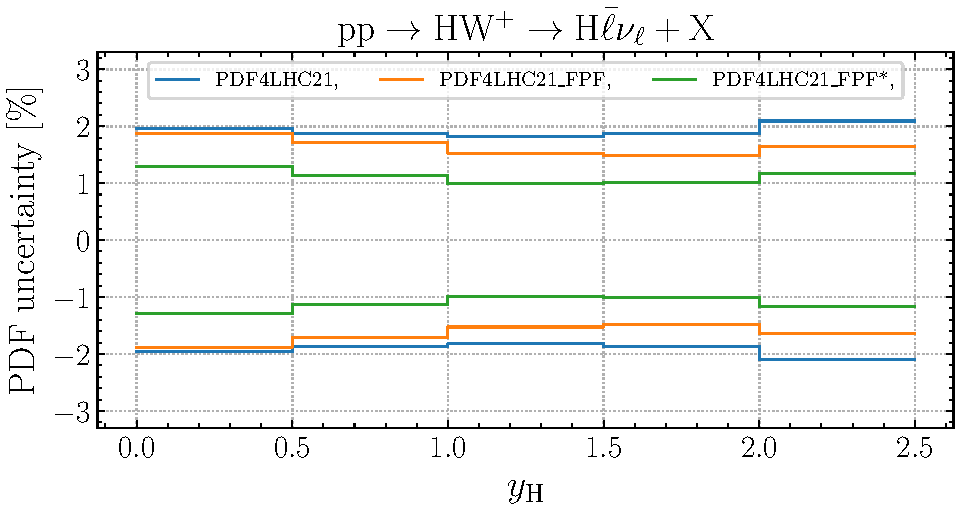
\includegraphics[width=0.49\textwidth]{plots/LHCpheno/NNPDF_HWP_14TEV_40_PHENO-global-pdf4lhc21.pdf}
	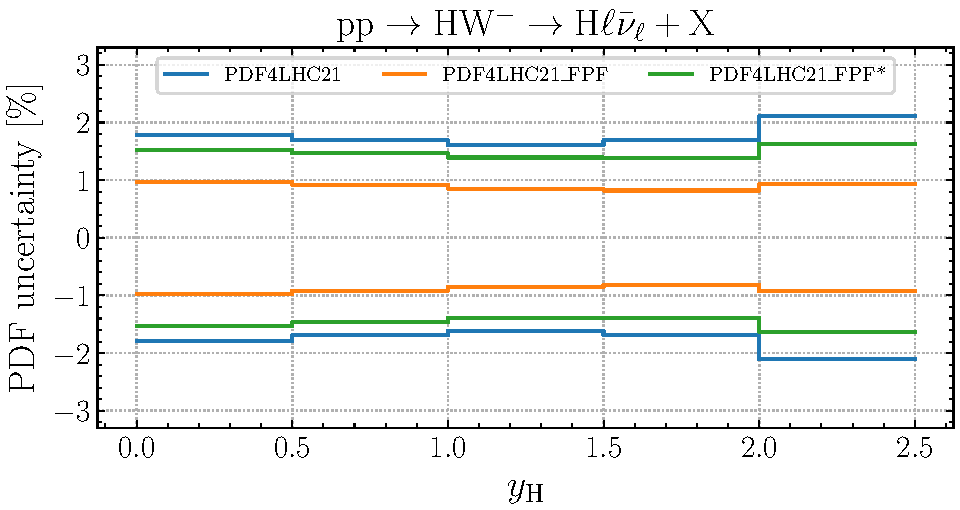
\includegraphics[width=0.49\textwidth]{plots/LHCpheno/NNPDF_HWM_14TEV_40_PHENO-global-pdf4lhc21.pdf}
	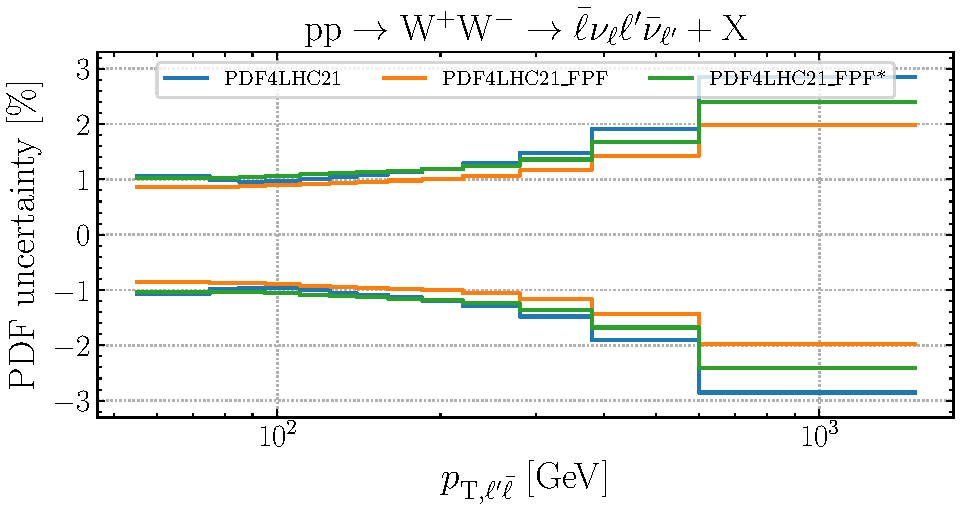
\includegraphics[width=0.49\textwidth]{plots/LHCpheno/NNPDF_WPWM_14TEV_40_PHENO-global-pdf4lhc21.pdf}
	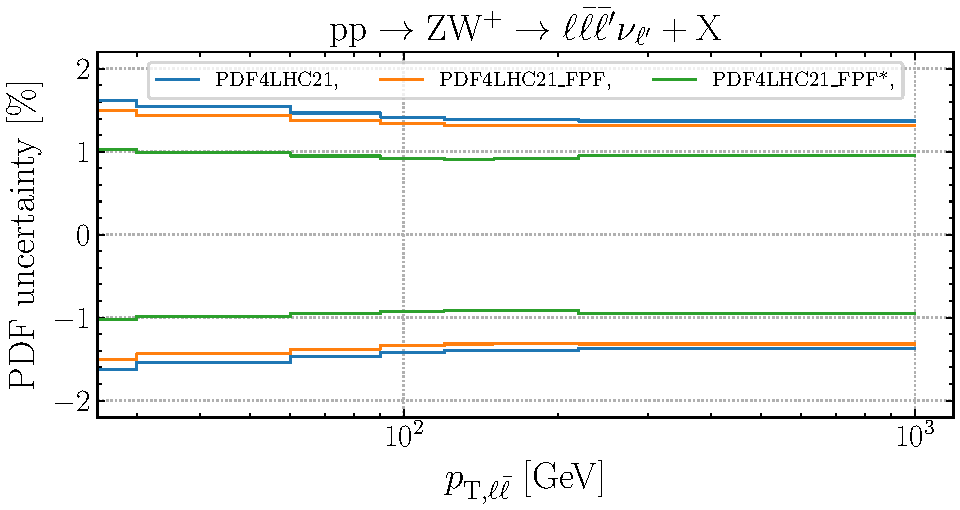
\includegraphics[width=0.49\textwidth]{plots/LHCpheno/NNPDF_WPZ_14TEV_40_PHENO-global-pdf4lhc21.pdf}
	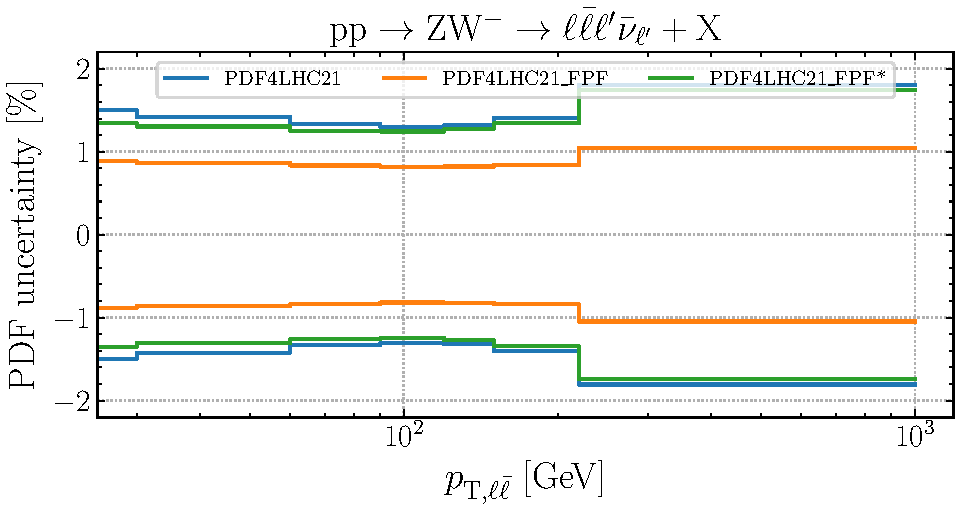
\includegraphics[width=0.49\textwidth]{plots/LHCpheno/NNPDF_WMZ_14TEV_40_PHENO-global-pdf4lhc21.pdf}
	\caption{
		Same as Fig.~\ref{fig:NNPDF40_pheno_differential} but with PDF4LHC21.
	}
	\label{fig:PDF4LHC21_pheno_differential}
\end{figure}
%%%%%%%%%%%%%%%%%%%%%%%%%%%%%%%%%%%%%%%%%%%%%%%%%%%%%%%%%%%%%%%%%%%%%%%%

Inspection of Figs.~\ref{fig:NNPDF40_pheno_integrated}--\ref{fig:PDF4LHC21_pheno_differential}
confirms the potential of LHC neutrino structure function measurements
to improve theoretical predictions for Higgs, electroweak and high-mass
processes at the HL-LHC.
%
In general, qualitative consistency between the results based on NNPDF4.0
and on PDF4LHC21 is found, as was already the case at the PDF level.
%
As  compared to the best-case scenario where only statistical uncertainties
are taken into account, the reduction of PDF errors in the LHC cross-sections
obtained thanks for the FPF structure functions becomes less marked,
but still visible for most of the processes under consideration,
upon the inclusion of systematic uncertainties in the fit covariance matrix.

Concerning the fiducial integrated cross-sections, a decrease in PDF
uncertainties is observed for all processes,
including for single gauge boson production relevant for core
HL-LHC analyses such as the $m_W$ and $\sin^2\theta_W$ measurements.
%
The specific improvement in precision depends
on the underlying scattering reaction as well as on the range
of $x$ and $Q^2$ covered by each process.
%
In the case of  Higgs associated production with vector bosons and in vector-boson
scattering,
driven by the quark-antiquark and quark-quark initial states respectively,
one observes that PDF uncertainties can  be reduced
by up to a factor two thanks to the FPF measurements, for instance
in the case of the $hW^+$ and $hW^-$ cross-sections,
in the most optimistic scenario in which systematic uncertainties
are neglected.
%
Likewise for the diboson cross-sections, with in this case the largest
improvement observed for the $ZW^+$  and  $ZW^-$ final states, with a reduction
of up to $\sim 40\%$ in the PDF uncertainties.

In the case of the differential cross-sections displayed in Figs.~\ref{fig:NNPDF40_pheno_differential}
and~\ref{fig:PDF4LHC21_pheno_differential},
one observes
how the impact of the FPF structure functions on LHC observables depends
on the hard-scattering scale.
%
For instance, searches for heavy resonances in the high-mass tail of the Drell-Yan
distributions could be improved by the addition of the FPF data.
%
Similar considerations apply for diboson prediction, and in the case of the $ZW^{\pm}$ channel we observe
an improvement specially in the low $p_{T,\ell\bar{\ell}}$ region which
represents the bulk of the fiducial cross-sections.
%
For the Higgs production processes, the PDF uncertainty in the theory predictions is relatively
stable as a function of the rapidity.
%
The effects of accounting for systematic uncertainties in the fit covariance
matrix are somewhat more visible here as compared to the inclusive cross-sections,
indicating that they affect mostly
the tails, rather than the bulk, of the distributions, and in particular the large-$x$
behaviour of the PDFs.
%
This observation emphasizes the importance of reducing systematic errors
in the FPF measurements in order to enhance the cross-talk with HL-LHC analyses.


